\documentclass[10pt,a4paper]{article}
\newcommand{\runningtitle}{Conditional flow matching in acute human wounds}
\usepackage[margin=15mm,top=16mm,bottom=17mm,headheight=12pt,headsep=5mm,footskip=9mm]{geometry}
\usepackage{fontspec}
\setmainfont{TeX Gyre Termes}
\setsansfont{Arial}
\usepackage{amsmath,amssymb,mathtools,bm}
\usepackage{unicode-math}
\setmathfont{TeX Gyre Termes Math}
\usepackage{graphicx,booktabs,array,tabularx,longtable}
% Keep captions visually separated from their artwork/table rules, while
% retaining a compact single-column manuscript.  The same defaults are used
% by both papers so appendix tables and main-text figures do not drift apart.
\usepackage[font=small,labelfont=normalfont,labelsep=period,skip=8pt]{caption}
\usepackage{flafter,placeins,needspace}
\usepackage[sort&compress,numbers]{natbib}
\usepackage[unicode,colorlinks=true,linkcolor=black,citecolor=black,urlcolor=black]{hyperref}
% longtable 4.24 uses infinitely shrinkable glue before a kernel box split.
% Backport the upstream 4.25 finite-shrink fix (latex3/latex2e issue 1907)
% locally. etoolbox is already loaded by hyperref; no runtime/package changes.
% Patch both nested vbox branches. Already-fixed versions are left unchanged.
\makeatletter
\patchcmd{\LT@output}{\vss}{\vskip\z@\@plus1fil\@minus\normalbaselineskip}{}{}
\patchcmd{\LT@output}{\vss}{\vskip\z@\@plus1fil\@minus\normalbaselineskip}{}{}
\makeatother
\usepackage{xcolor,microtype,titlesec,enumitem,fancyhdr}
\usepackage{bookmark}
\hypersetup{pdfcreator={XeLaTeX},pdfauthor={Zeyu Fu}}
\graphicspath{{figures/}}
\setlength{\parindent}{1em}
\setlength{\parskip}{1pt plus .4pt}
\linespread{1.02}
\setlength{\textfloatsep}{12pt plus 2pt minus 1pt}
\setlength{\floatsep}{10pt plus 2pt minus 1pt}
\setlength{\intextsep}{12pt plus 2pt minus 1pt}
\renewcommand{\topfraction}{.94}
\renewcommand{\bottomfraction}{.88}
\renewcommand{\textfraction}{.06}
\renewcommand{\floatpagefraction}{.78}
\setcounter{topnumber}{3}
\setcounter{bottomnumber}{2}
\setcounter{totalnumber}{4}
\setlength{\abovedisplayskip}{4pt plus 1pt minus 2pt}
\setlength{\belowdisplayskip}{4pt plus 1pt minus 2pt}
\setlength{\abovedisplayshortskip}{2pt plus 1pt}
\setlength{\belowdisplayshortskip}{3pt plus 1pt}
\titlespacing*{\section}{0pt}{8pt plus 1pt minus 2pt}{3pt}
\titlespacing*{\subsection}{0pt}{6pt plus 1pt minus 1pt}{2pt}
\titleformat{\section}{\large\bfseries}{\thesection}{.6em}{}
\titleformat{\subsection}{\normalsize\bfseries}{\thesubsection}{.6em}{}
\setlist{nosep,leftmargin=1.7em,topsep=4pt}
\setlength{\bibsep}{1.5pt}
\renewcommand{\bibfont}{\small\let\emph\textnormal}
\setlength{\tabcolsep}{4pt}
% Longtable captions sit above the first rule.  These pre/post skips prevent
% adjacent appendix tables from reading as one continuous table while still
% allowing a continued table head to remain visually attached to its rows.
\setlength{\LTpre}{8pt plus 2pt minus 1pt}
\setlength{\LTpost}{8pt plus 2pt minus 1pt}
\setlength{\LTcapwidth}{\textwidth}
\captionsetup[figure]{skip=8pt}
\captionsetup[table]{skip=8pt}
\captionsetup[longtable]{font=footnotesize,skip=8pt}
\renewcommand{\arraystretch}{1.12}
\setlength{\emergencystretch}{1.2em}
\widowpenalty=10000
\clubpenalty=10000
\raggedbottom
\pagestyle{fancy}
\fancyhf{}
\fancyhead[L]{\sffamily\fontsize{8}{10}\selectfont\runningtitle}
\fancyfoot[C]{\small\thepage}
\renewcommand{\headrulewidth}{.25pt}
\newcommand{\papertitle}[1]{\thispagestyle{plain}\begin{center}\vspace*{-5mm}{\fontsize{19}{22}\selectfont\bfseries #1\par}\vspace{2mm}{\normalsize Zeyu Fu\par}\end{center}\vspace{-2mm}}
\newcommand{\paperfigure}[3]{\begin{figure}[!htbp]\centering\includegraphics[width=\linewidth]{#1.pdf}\caption{#3}\label{#2}\end{figure}}
\newcommand{\supplement}{\FloatBarrier\section*{Supplementary methods and numerical results}\addcontentsline{toc}{section}{Supplementary methods and numerical results}\setcounter{section}{0}\setcounter{table}{0}\setcounter{equation}{0}\renewcommand{\thesection}{S\arabic{section}}\renewcommand{\thetable}{S\arabic{table}}\renewcommand{\theequation}{S\arabic{equation}}\renewcommand{\theHsection}{supp.\arabic{section}}\renewcommand{\theHtable}{supp.\arabic{table}}\renewcommand{\theHequation}{supp.\arabic{equation}}}
\newcolumntype{L}{>{\raggedright\arraybackslash}X}
\newcommand{\doi}[1]{\href{https://doi.org/#1}{doi: #1}}
\newcommand{\E}{\mathbb{E}}
\newcommand{\R}{\mathbb{R}}
\newcommand{\ind}{\mathbf{1}}

% Keep the enlarged Results figures with substantive text instead of creating
% early, vertically centred float-only pages. Barriers still flush pending art.
\hypersetup{pdftitle={Conditional flow matching in acute human wounds: a three-donor audit of population reconstruction}}

\title{Conditional flow matching in acute human wounds: a three-donor audit of population reconstruction}
\author{Zeyu Fu$^{1,*}$\\[3pt]\small $^1$State Key Laboratory of Trauma and Chemical Poisoning,\\\small Institute of Combined Injury, Chongqing Engineering Research Center for Nanomedicine,\\\small College of Preventive Medicine, Army Medical University, Chongqing, China\\\small $^*$Correspondence: \texttt{fuzeyu09@gmail.com}; \texttt{fuzeyu99@126.com}}\date{}
\usepackage{float}
\usepackage[switch]{lineno}
\begin{document}
\maketitle
\modulolinenumbers[5]\linenumbers
\begin{abstract}
Models of changing cell populations can reproduce an observed distribution without learning motion that improves prediction. We tested this distinction in acute human wounds from three donors sampled at four times. A conditional flow model was evaluated both when a sampling time was omitted across all donors and when an entire donor was excluded from training. Its predictions improved over leaving the starting population unchanged, but simpler permitted controls often performed better. Other donors' observed target distributions beat the flow in two of the three held-donor comparisons, and simple interpolation was competitive for missing times. Training-fitted principal-component controls also showed no consistent flow advantage, reducing reliance on the expression encoder transferred from another disease dataset. Changes to the time coordinate, representation and model selection did not resolve the baseline concern. These results show why unchanged-source comparisons alone can overstate evidence for learned population motion. The study supports a conditional reconstruction assessment, with uncertainty limited by three donors; it does not identify individual cell trajectories or establish clinical prognosis.
\end{abstract}
\noindent\textbf{Keywords:} flow matching; wound healing; population prediction; donor transfer; time coordinates; single-cell analysis.

\section{Introduction}
Wound repair involves changing populations of inflammatory, stromal and epithelial cells, together with changes in the activity of those cells \citep{wilkinson2020}. Experimental studies show that fibroblast proliferation, matrix deposition and interactions with macrophages contribute to the organization of repairing skin \citep{rognoni2018,shook2018}. These processes motivate a temporal description of wound tissue, but they do not imply that all wounds follow a common transcriptional clock. Acute repair in healthy skin and the course of a diabetic foot ulcer differ in their clinical setting, and a model of one cannot be assumed to predict the other \citep{armstrong2017}.

Single-cell sequencing provides detailed observations of these populations while destroying the cells being measured. Samples collected at successive times therefore describe distributions of cell states rather than repeated observations of individual cells. More than one dynamic process can connect the same marginal distributions, which limits what can be identified from snapshots alone \citep{weinreb2018}. Combining transcriptional profiles with experimental lineage tracing can connect state to subsequent fate and supply information absent from expression snapshots \citep{weinreb2020}. Without such information, a smooth computational trajectory should be interpreted in terms of its stated assumptions and prediction target.

Different single-cell methods use different sources of temporal information. Trajectory inference organizes cells according to a modeled state-space topology or progression \citep{saelens2019}. RNA velocity uses spliced and unspliced transcript information to estimate local expression change, with dynamical extensions relaxing particular steady-state assumptions \citep{lamanno2018,bergen2020}. CellRank combines local directional information with a probabilistic description of fate transitions \citep{lange2022}. These approaches address questions related to, but distinct from, predicting the distribution of cells recovered from a later tissue specimen. Their outputs cannot be treated as equivalent observations of longitudinal biological motion.

Distributional models instead specify how one population measure is related to another. Optimal transport uses a chosen cost and coupling to connect observations \citep{schiebinger2019,peyre2019}, while neural differential equations represent a continuous evolution in state space \citep{chen2018ode,tong2020trajectory}. Flow matching learns a vector field from a prescribed family of paths and conditional regression targets \citep{lipman2023,tong2023,lipman2024guide}. The primary neural field uses a product endpoint coupling rather than the minimum-kinetic-energy transport construction \citep{benamou2000}. Its non-neural comparator uses entropic transport via Sinkhorn optimization and the Python Optimal Transport implementation \citep{cuturi2013,flamary2021}. Additional neural fits change the endpoint coupling to transport or a stochastic bridge to assess dependence on that choice. Neural stochastic differential equations additionally model diffusion, with recent work evaluating such models against lineage-informed trajectories \citep{vinyard2025}. Related transport models have also been used for perturbation prediction \citep{bunne2023}. These developments expand the modeling choices; they do not remove the need to test whether a selected model predicts observations withheld from its construction.

That test depends on what is withheld. Removing one time point from every donor asks whether the model can reconstruct an unobserved part of the temporal sequence. Removing one donor while retaining all times in the others asks whether relationships learned from those donors transfer to the excluded person. In the latter setting, the observed source distribution of the test donor can initialize prediction without supplying its target. Neither design is equivalent to randomly separating cells from the same specimens. Cross-validation for structured data needs to reflect the dependence and extrapolation relevant to the intended application \citep{roberts2017}. The prediction task therefore has to be defined before model performance can be interpreted.

The biological object of prediction should also be made explicit. An observed fibroblast distribution is recovered from one sampled tissue region at one time; its transcriptional variation can reflect activation, composition within the compartment and technical recovery \citep{rognoni2018,heumos2023}. Descriptive expression profiles help connect latent coordinates to that material without converting the coordinates into a spatial wound map. A mean translation between available samples provides a particularly direct baseline: it asks whether moving the center of the observed population is sufficient for the evaluated target, before attributing predictive value to a flexible nonlinear field \citep{schiebinger2019}. Such a baseline must receive the same permitted donor and temporal information as the model it is compared with.

Evaluation also depends on the representation and probability measure being compared. A latent expression map makes distributional calculations tractable but determines which differences contribute to distance \citep{lopez2018}. Quality control and normalization also determine which cells and variation enter that comparison \citep{heumos2023}. Experience with atlas integration shows that preserving biological variation and removing technical differences can be competing objectives \citep{luecken2022}. Energy distance supplies a distributional discrepancy with established connections to kernel-based testing \citep{szekely2013,sejdinovic2013}, but a distance in latent coordinates is not automatically a distance in clinical severity or gene-specific function. Pooling cells weights donors according to their recovered cell counts unless weights are changed explicitly. Preprocessing, weighting and a simple unchanged-source baseline are consequently part of the prediction question rather than incidental implementation choices.

The number of independent donors constrains what repeated computational evaluation can establish. Many cells improve the empirical description of each sampled population, while leaving donor-level biological replication unchanged \citep{zimmerman2021}. Training seeds, integration resolutions and cell-sampling draws examine other sources of variability. Model selection on the same small held-out set can still lead to optimistic estimates, even when the fitting procedure is reproducible \citep{varma2006,cawley2010}. Small-sample validation studies also show why performance estimates require caution when the data support many analytical choices but few independent test units \citep{vabalas2019}. These considerations favor a clearly bounded reconstruction task with explicit controls over a claim of unrestricted clinical generalization.

The acute human wound atlas supplies four measurement times from three healthy volunteers \citep{liu2025_wound,geo_gse241132}. The expression representation is frozen from a separate public diabetic-foot skin dataset, not learned from the acute-wound evaluation targets \citep{theocharidis2022}. We use this setting to ask whether moving an observed day-1 distribution under a fitted field brings it closer to held-out day-7 cells than leaving the source unchanged or using the other permitted observations directly. Separate timepoint and donor exclusions define the two prediction tasks. Comparisons of time coordinates, shared and donor-conditioned fields, non-neural predictors, training-donor counts and seeds examine the dependence on modeling choices. Fixed-field integration, evaluation sampling and donor weighting address additional computational and measurement choices. Public mouse time courses provide a separate computational comparison under different biological and replication conditions \citep{geo_gse326622}. The aim is to establish what this limited design can test about distributional prediction before extending its interpretation to individual wound progression.

\section{Results}
\subsection{Cross-sectional observations define two different reconstruction questions}
The study compared predicted cell populations with public acute-wound measurements from three donors at four times. The information available to a globally missing-time model differs from that available when a donor is held out (Figure~\ref{fig:p2f1}a). The observed cells vary by time, donor and expression, while their numbers do not increase the donor count (Figure~\ref{fig:p2f1}b--e). Displayed numerical paths transport starting coordinates and are not observed cell fates (Figure~\ref{fig:p2f1}f).

\begin{figure}[H]\centering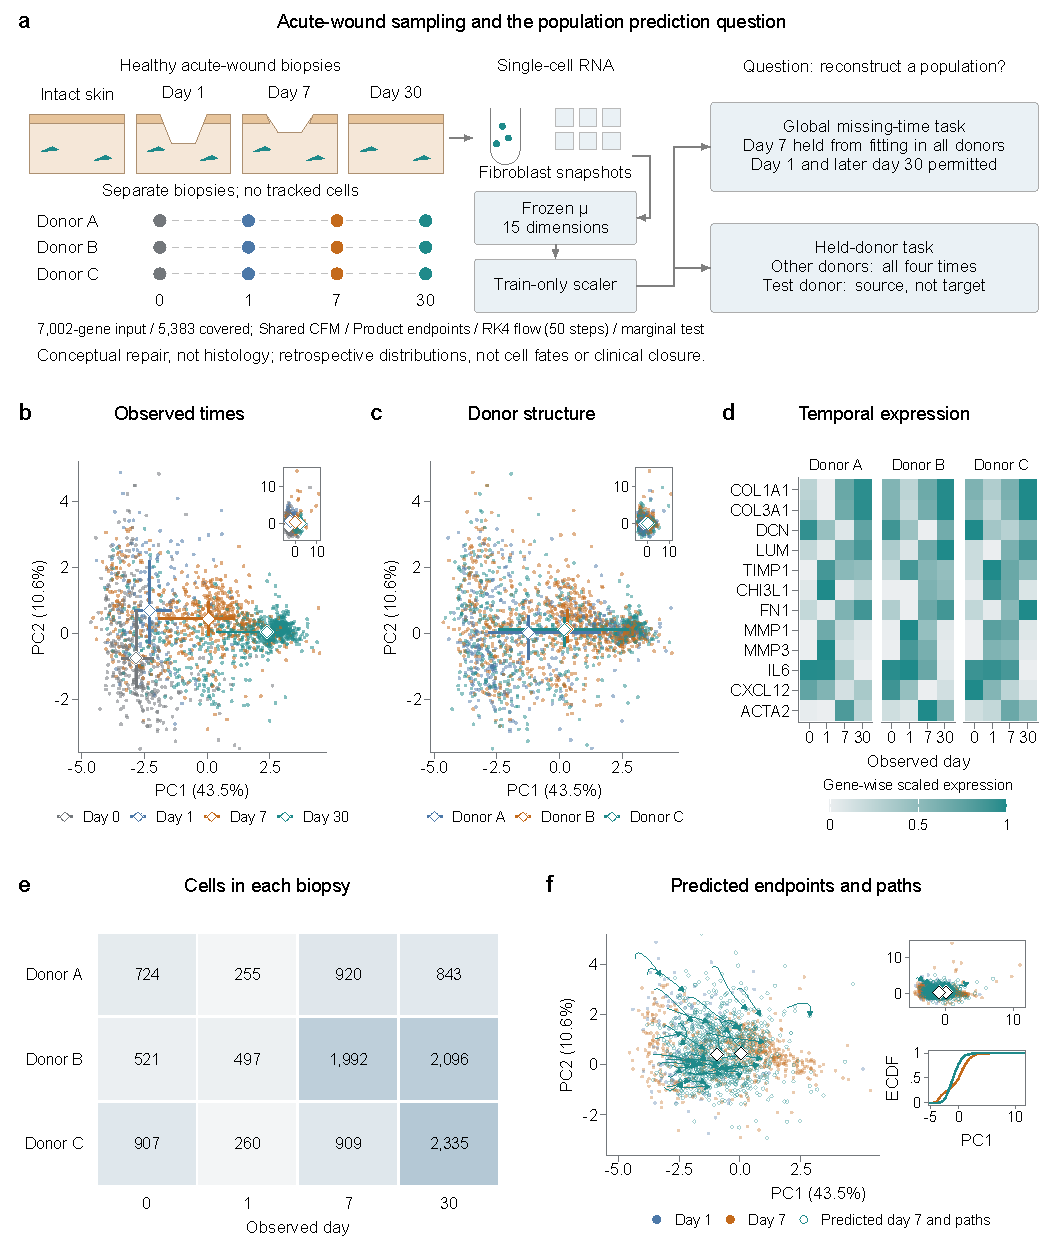
\includegraphics[width=\linewidth]{journal-figures/paper2_figure1_workflow.pdf}
\caption{What can acute-wound snapshots predict? (a) Conceptual repair and separate biopsies from three healthy donors at days 0, 1, 7 and 30; cells are not tracked. Global missing-time reconstruction excludes day 7 in every donor and permits later anchors. Held-donor transfer permits training-donor day-7 cells but excludes the test donor's target. Neither is clinical prognosis. A 7,002-gene input with 5,383 covered genes feeds frozen 15-dimensional μ, training-only scaling, product-endpoint CFM and 50-step RK4. Flow acts in scaled μ coordinates, not simplex weights. (b) Saved 2,000-cell display by time; day-7-excluded PCA explains 43.5\% and 10.6\% of training variance. (c) The same cells by donor. Diamonds/crosses denote medians/interquartile spans, not confidence intervals; focus windows retain full-range insets. (d) Twelve measured genes per biopsy, gene-wise scaled after pseudobulk normalization. (e) Recovered fibroblasts, not independent donors. (f) All 1,012 saved seed-0 endpoints, 36 numerical paths and observed day-1/day-7 display; insets show full range and PC1 cumulative distributions. Paths are not cell fates; errors use all 15 coordinates.}\label{fig:p2f1}\end{figure}
\FloatBarrier

Flow improved over leaving the observed source unchanged in the original global day-7 comparison and in each held-donor fold (Figure~\ref{fig:p2f2}a,b). The global relative improvement was 49.9\%, and the mean held-donor relative improvement was 75.9\%. These point comparisons show that the fitted model can approach a target more closely than an unchanged source. They do not show that learning a motion improves on the target information already available during training. Donor--time geometry also differed across the observed populations (Figure~\ref{fig:p2f2}c), limiting a single pooled interpretation.

\begin{figure}[H]\centering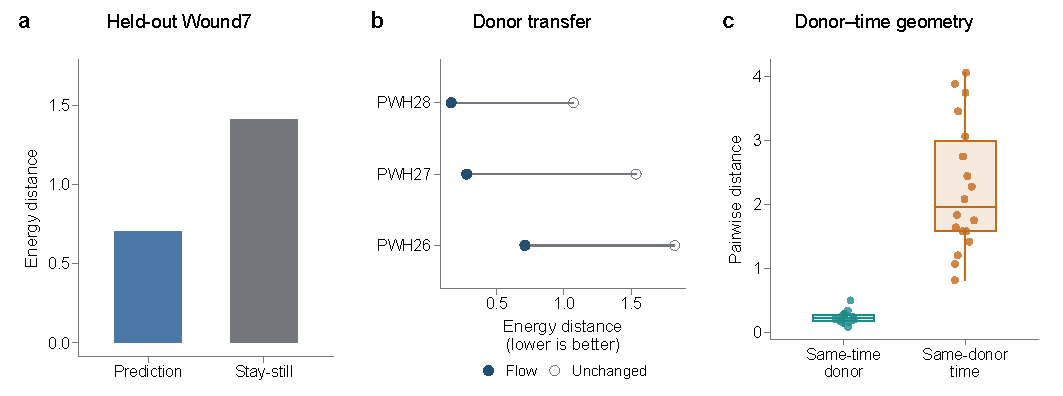
\includegraphics[width=\linewidth]{journal-figures/paper2_figure2_wound7_transfer.pdf}
\caption{Global Wound7 reconstruction, donor transfer and donor--time geometry. (a) Predicted and unchanged-source energy distances to pooled Wound7 after excluding that time globally; relative improvement is 49.9\%. (b) Connected filled and open points give predicted and unchanged-source errors for each genuinely excluded donor; the other two donors retain all four times. Mean relative improvement is 75.9\%, but absolute baseline and prediction errors differ by donor. These are point estimates, not confidence intervals. (c) Twelve same-time between-donor and 18 same-donor between-time distances, with interquartile boxes, medians and whiskers to observations within 1.5 interquartile ranges. The median temporal/donor ratio is 8.46; its 10,000-draw pair-distance resampling range is descriptive. All distances use training-standardized latent coordinates. Shared donors make pairs dependent, so these ranges have no established population coverage; three healthy donors do not validate DFU prediction.}\label{fig:p2f2}\end{figure}
\FloatBarrier

\subsection{Simple interpolation competes with flow when a time is missing}
For both global day-7 and day-1 holdouts, permitted observed times supplied anchors for simple interpolation (Figure~\ref{fig:p2f3}a,b). Mean displacement and location--scale predictions were competitive with the neural model. Donor-specific contrasts and seed sensitivities retained the comparisons rather than replacing them with a pooled winner (Figure~\ref{fig:p2f3}c,d). Centered distributions and paired sampling draws supplied separate shape and sampling sensitivities (Figure~\ref{fig:p2f3}e,f); these repeats do not create biological confidence intervals. This is retrospective reconstruction: later observed populations are available as anchors, so the task is not source-only clinical prediction.

\begin{figure}[H]\centering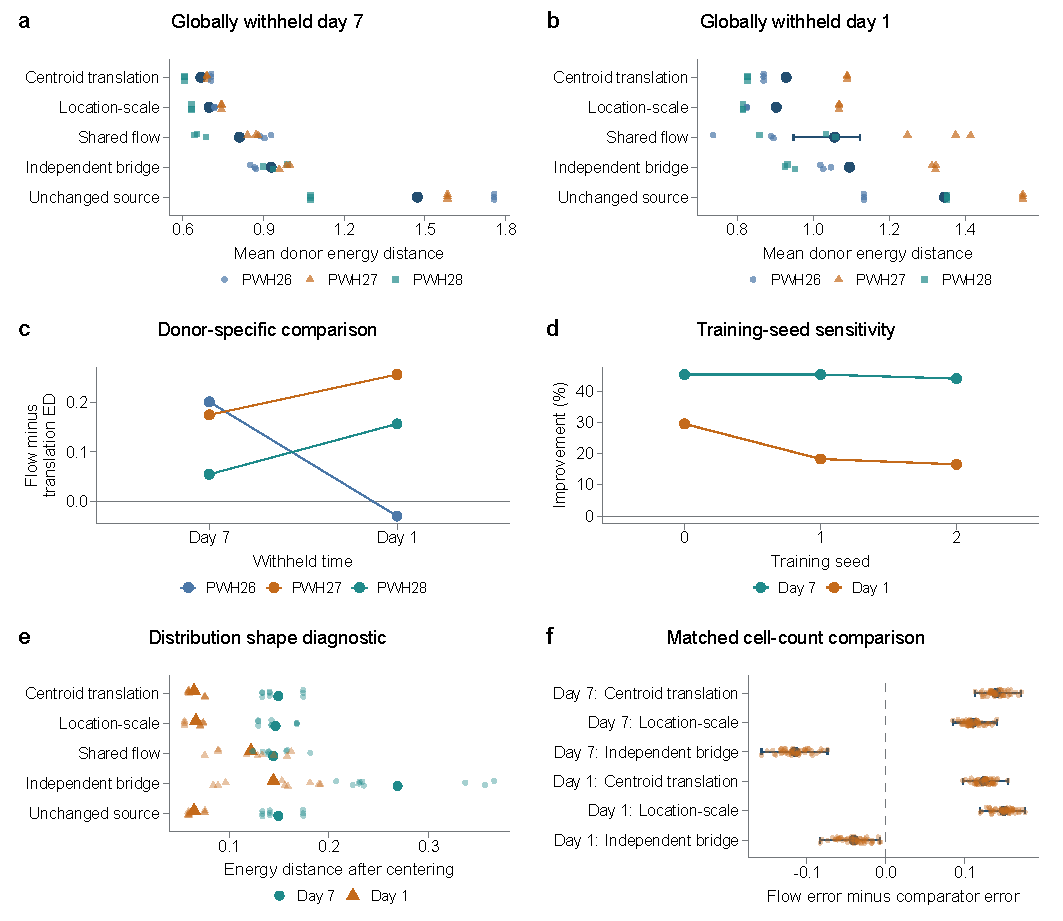
\includegraphics[width=\linewidth]{journal-figures/paper2_figure3_interpolation_controls.pdf}
\caption{Simple baselines for globally missing times. (a) Day 7 from day 1 with observed day 30 as anchor. (b) Day 1 from intact skin with observed day 7 as anchor. Large points are donor-macro means and bars span three seeds; smaller colored symbols retain individual donor/seed errors for all five predictors, including location--scale. Both tasks use rank-time fraction one half and are retrospective interpolation, not source-only prediction. (c) Donor-specific seed-averaged flow-minus-translation error. (d) Each flow seed's relative improvement. (e) Seed/donor-averaged centered energy distance with the individual donor/seed errors behind it; this is a shape diagnostic rather than additive error decomposition. (f) All 50 saved donor/seed-averaged paired draw contrasts, overlaid with means and ranges, using 200 source and target cells per donor. Positive differences favor the comparator. Seeds and draws are dependent computational evaluations of three donors; neither their ranges nor their point clouds are biological confidence intervals.}\label{fig:p2f3}\end{figure}
\FloatBarrier

\subsection{Training-target marginals beat flow in two held donors}
The sharper held-donor comparison used the observed target populations of the two training donors as a predictor. Its equal-donor mean error was 0.1818, compared with 0.3947 for the shared flow field (Figure~\ref{fig:p2f5}a). Donor conditioning improved fits to the training donors (Figure~\ref{fig:p2f5}b).

\begin{figure}[H]\centering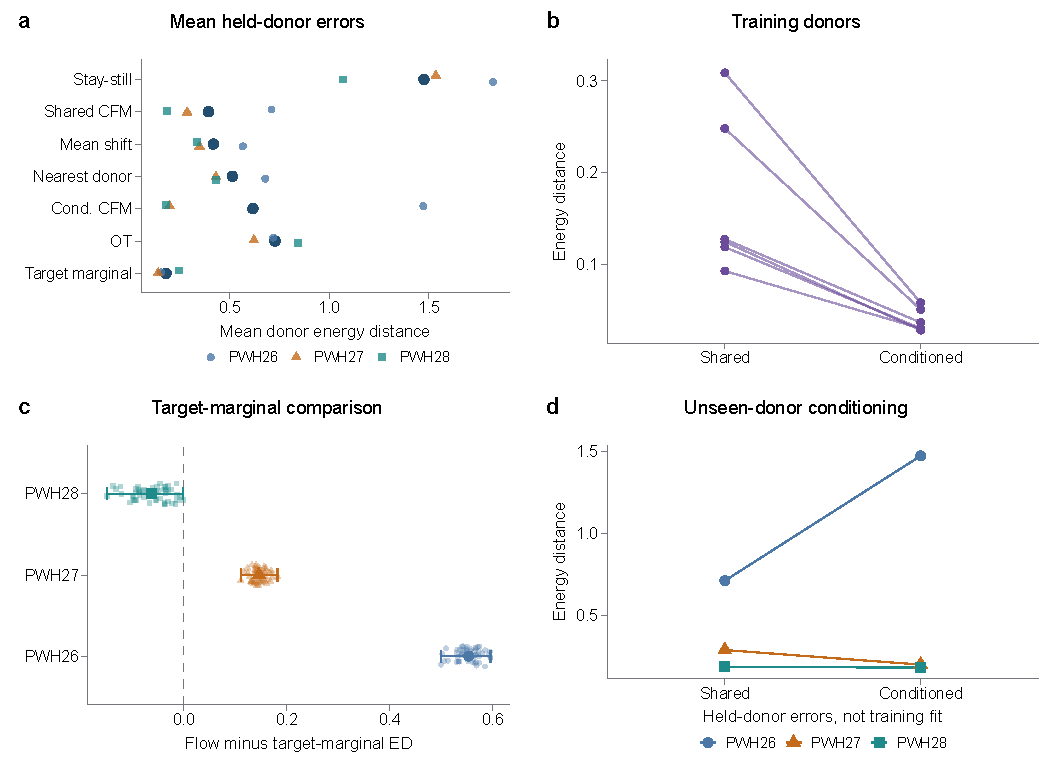
\includegraphics[width=\linewidth]{journal-figures/paper2_figure5_methods_benchmark.pdf}
\caption{Method means and donor-specific reversals in the historical held-donor benchmark. (a) Navy points are equally donor-weighted mean energy distances for unchanged source, five predictors and the added target marginal; smaller colored points retain all three donor errors for each method. CFM is conditional flow matching; OT is the separate entropic transport comparator. The marginal assigns equal mass to training-donor day-7 distributions without held-source expression; 50 matched-particle draws use the original target rows and scaling. (b) Six shared-versus-conditioned comparisons on training donors, all favoring conditioning; these are overlapping training observations, not transfer tests. (c) Each donor's fixed shared-field error minus the marginal's mean error, with the full 50-draw range and all 50 saved contrasts as smaller points. Positive values favor the marginal; PWH28 instead favors the field. These ranges describe prediction sampling, not donor-population confidence. (d) Connected shared and conditioned errors for the three genuinely held donors, separately exposing the gap between training fit and unseen-donor behavior. Historical neural/transport predictors used one training seed; the retrospective marginal audit does not establish a stable method ranking.}\label{fig:p2f5}\end{figure}
\FloatBarrier

The target-marginal errors for PWH26, PWH27 and PWH28 were 0.1569, 0.1416 and 0.2469, whereas the shared-field errors were 0.7110, 0.2881 and 0.1850. Thus the simpler predictor was better in two of three donors, with a reversal in the third (Figure~\ref{fig:p2f5}c).

Donor conditioning did not establish a corresponding held-donor advantage (Figure~\ref{fig:p2f5}d). The target marginal uses no expression values from the held donor's observed source. Its performance shows why improvement over an unchanged source alone is insufficient evidence that the learned motion is useful for this transfer task. Evaluation draws describe sampling sensitivity within the same three donors.

\subsection{Repeated controlled comparisons preserve donor-specific outcomes}
Comparisons using a common scoring geometry and symmetric computational budgets retained the baseline concern. Missing-time ratios compare flow with permitted translation, while held-donor ratios compare it with the observed training-target marginal (Figure~\ref{fig:p2f8}a,b). Near-parity and contrary results remained visible. Replacing the starting population within a fixed fitted field showed that reconstruction also depended on its supplied source (Figure~\ref{fig:p2f8}c). Fitting-cost summaries counted jobs once and did not treat runtime or repeats as additional evidence from donors (Figure~\ref{fig:p2f8}d).

\begin{figure}[H]\centering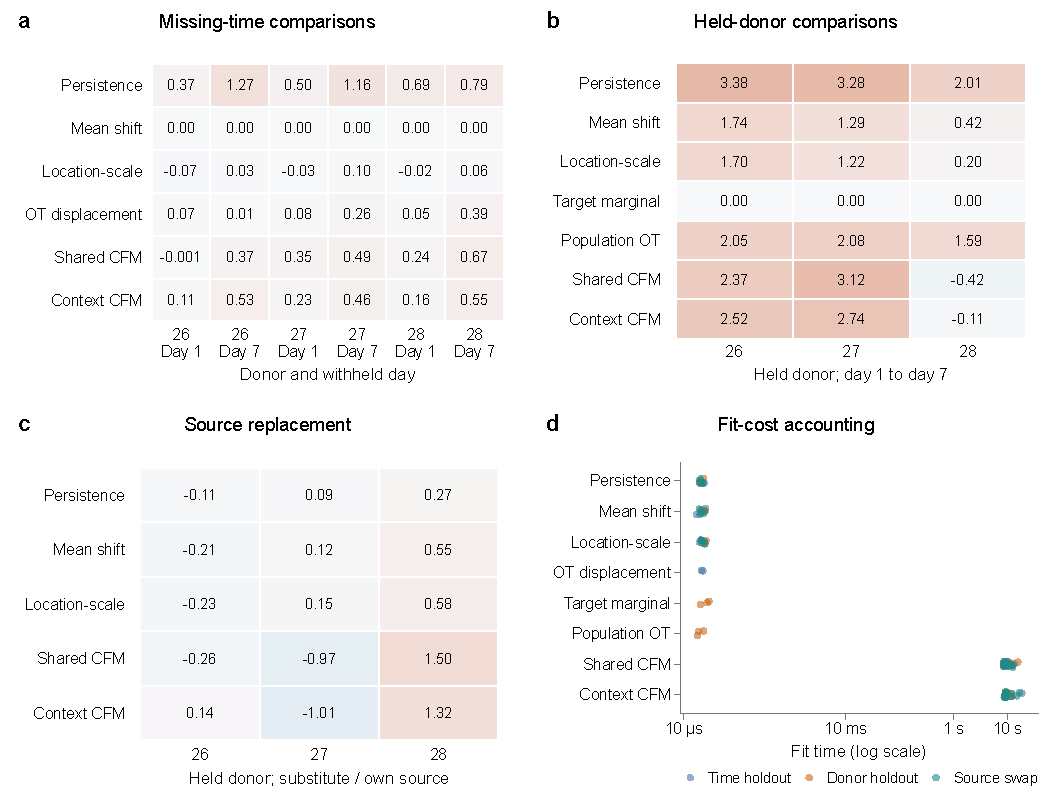
\includegraphics[width=\linewidth]{journal-figures/paper2_figure8_paired_comparison.pdf}
\caption{Source-bound repeated comparisons in the frozen representation. (a) Each cell is the mean paired log2 energy-error ratio to mean translation within a donor and withheld day, averaging 50 matched draws within a fit and then three neural training seeds. (b) Day-1-to-day-7 donor-transfer ratios use the permitted equal-training-donor target marginal instead. Negative values favor the row method; zero denotes its comparator. Neither display pools raw distances from differently standardized donor folds. (c) Source replacement divides each substituted-source error by the own-source error from the same field and target draw, then averages draws, seeds and the two substitute choices within donor. These separate fits exclude both the held donor and the substitute from fitting; positive values indicate lower error from the own source. (d) Every one of the 107 fitted-job timings is counted once, not once per evaluation draw; colors distinguish missing-time, held-donor and source-replacement tasks. Fit time excludes representation setup, prediction, scoring and input/output and is not an equal-compute comparison. Original-CUDA-backend replay and the failed CPU portability check are distinguished. All panels reuse three healthy acute-wound donors, without inferential method ranking or clinical validation.}\label{fig:p2f8}\end{figure}
\FloatBarrier

The complete follow-up includes the common-reference donor-count comparison, paired clocks, evaluation draws and numerical-resolution sensitivities. These changes separate the scoring scale from the training information set; they do not resolve the small biological sample.

\subsection{Training-fitted geometry controls do not remove the baseline concern}
Changing endpoint coupling altered missing-day-7 errors without establishing a consistent neural advantage (Figure~\ref{fig:p2f9}a). Across all five coordinate systems, the donor-mean day-7 comparison favored translation over both independently coupled and transport-coupled flow (Figure~\ref{fig:p2f9}b). This panel includes principal components fitted only to training cells. The baseline concern therefore persisted beyond the incomplete expression panel transferred from a diabetic-foot dataset, although representation transfer remains a limitation.

\begin{figure}[H]\centering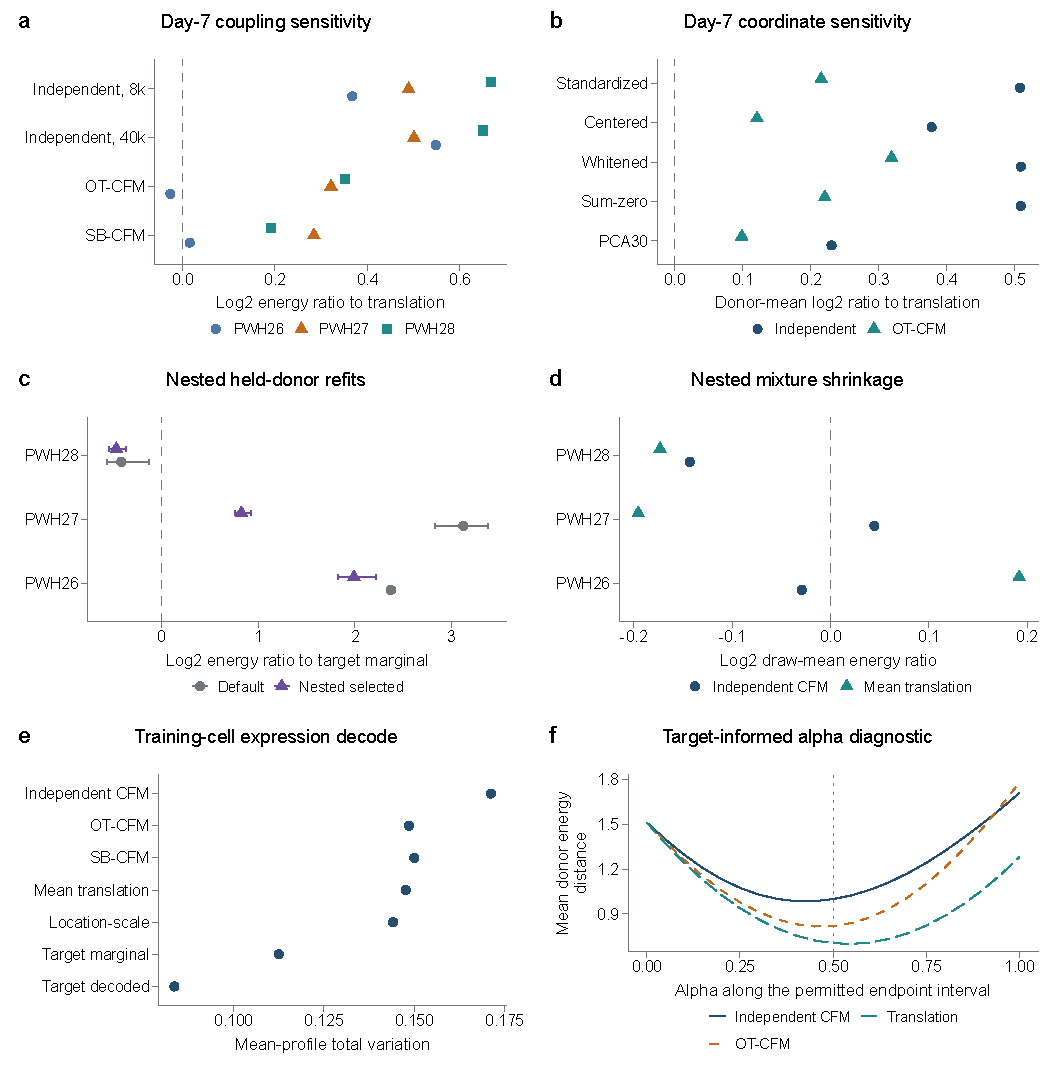
\includegraphics[width=\linewidth]{journal-figures/paper2_figure9_followup.pdf}
\caption{Completed computational follow-up. (a) Missing-day-7 log2 energy ratios to translation in each donor, across coupling families and two independent-field budgets. (b) Donor-mean day-7 ratios in five training-fitted coordinate systems. (c) Default and nested selected day-1-to-day-7 fields relative to the training target marginal; whiskers span three seed means. (d) Nested mixtures of transported source and target marginal, using log2 ratios of draw-averaged energies, a different estimand from a--c. (e) Held-donor mean-expression errors after mapping predictions to 15 nearest permitted training cells; decoding observed target cells supplies a reference. (f) Target-informed alpha scans of fixed rank-trained predictors, with rank alpha 0.5 dotted. Alpha optima are retrospective diagnostics. All panels reuse three human donors; draws and seeds add no biological replication.}\label{fig:p2f9}\end{figure}
\FloatBarrier

Nested selection reduced errors relative to the default field within every donor but left the target-marginal comparison donor-specific (Figure~\ref{fig:p2f9}c). Mixtures with the permitted marginal also retained contrary comparisons (Figure~\ref{fig:p2f9}d). Decoded expression errors did not establish an advantage over the marginal; decoding measured coordinates itself introduced mismatch (Figure~\ref{fig:p2f9}e). The target-informed mixture scan is a descriptive envelope, not a held-out selection result (Figure~\ref{fig:p2f9}f).

Saved CUDA predictions and selected coordinate calculations were reproduced, while the complete CPU reintegration and retrospective training-provenance gaps remained unresolved. Separate mouse analyses characterize protocol sensitivity and are reported with their animal-count limitations in the supplement. The collective result is a bounded assessment of population reconstruction: a learned flow can improve on unchanged source without consistently beating permitted simple predictors or identifying individual trajectories.



















\section{Discussion}

Coupling variants and nested model selection qualify the interpretation of the default neural field. The completed outer refits reduced its errors, but selected fields still lost to the training target marginal in two of three held donors and improved in the third.

The symmetric repeated comparison confirms the baseline concern without making it universal. Missing-day-7 reconstruction favored mean translation in every neural donor--method mean, while held-donor day-7 reconstruction favored neural fields over the target marginal for PWH28 but not PWH26 or PWH27.

The global missing-time comparison changes the interpretation of model complexity. A within-donor mean translation had lower average error than the shared field for both withheld times, even though the field improved over an unchanged source.

The donor-holdout task exposes a further baseline requirement. Because the target time is observed in training donors, their empirical target distributions can supply a prediction without using the excluded donor's starting expression.

The observed-cell maps and biopsy expression profiles make the population being transported more concrete, but they do not establish a lineage or wound mechanism. A two-dimensional projection omits variation even when fitted solely to training cells \citep{huang2022visualization}.

The learned field is a model of distributions under a specified sampling construction. Independent endpoint cells from the same donor define linear paths and regression targets; those pairings are not observed cell lineages or an estimated minimum-cost coupling.

Additional biological measurements would constrain a different part of the problem. Lineage tracing relates ancestry to later cell states, whereas RNA velocity derives directional information from transcript processing under a kinetic model \citep{weinreb2020,lamanno2018,bergen2020}.

Normalization to a probability distribution introduces another biological limit. Wound repair involves proliferation, loss, recruitment and matrix remodeling, with experimental evidence for coordinated fibroblast and macrophage responses \citep{rognoni2018,shook2018}.

The time-axis comparison identifies a consequential modeling choice. The revised three-seed audit pairs the random streams and integrates to the exact target, addressing defects in the original single-seed comparison.

Donor conditioning improved the fit to known donor contexts without improving the overall held-out mean relative to the shared field. Additional context can increase fitting capacity while also creating an extrapolation problem for an unfamiliar donor.

The distance used for evaluation also determines the interpretation of improvement. Energy distance compares distributions through pairwise geometry and has a formal relationship to kernel discrepancies \citep{szekely2013,sejdinovic2013}.

The fitted and evaluated donor measures also differ. Cycling through donor--segment pairs approximately balances training contributions, whereas pooled evaluation weights cells according to yield.

Numerical integration and evaluation sampling were stable over the tested settings for one fixed field. Increasing Runge--Kutta resolution changed the coordinates negligibly, and repeated subsampling preserved improvement.

The finite-budget train-PCA diagnostic extends the baseline concern across multiple coupling variants and both budgets in all three donors. It remains a separate experiment: preprocessing, architecture, intervals and optimization settings differ from the primary frozen-coordinate analysis.

An external mouse series was admitted narrowly. Three of four arm and gate tasks failed the frozen 50-cell floor at the last time point, and the unwounded and POD2 libraries could not be assigned because no hashtag counts were released.

The mouse arms had different errors, one animal per time and incomplete panel coverage; time, animal and representation effects remain entangled. Neither acute human nor mouse wounds supply independently observed diabetic-foot-ulcer courses \citep{armstrong2017}.


\section{Methods}
\subsection{Cohort and representation}
GSE241132 supplied three healthy acute-wound donors, sampled at intact skin and days 1, 7 and 30. Joining the original sample and cell identities yielded 12,259 author-annotated fibroblasts for temporal analysis. The frozen expression encoder was trained on a diabetic-foot dataset, GSE165816. It mapped normalized counts to a 15-dimensional Gaussian mean coordinate, with 5,383 of its 7,002 panel genes covered in the acute-wound input. Absent panel genes were zero-filled. Scaling was fitted on training cells only. The incomplete transferred panel is a limitation, so separately fitted principal-component representations were included as controls.

\subsection{Two distinct prediction tasks}
Global missing-time reconstruction excluded day 7 from every donor before fitting and scaling. Observed later times could serve as anchors, making this retrospective interpolation rather than source-only prognosis. Held-donor transfer excluded every cell of the test donor from model fitting and scaling while allowing the other donors' day-7 distributions. The test donor's observed source supplied starting cells but its target was reserved for evaluation. These information sets were kept separate.

Conditional flow matching fitted a time-dependent velocity field to bridges between permitted observed populations. The recorded architecture, coupling, optimization budgets, clocks and integration settings are specified in the Supplementary Methods. Predictions describe transported populations; cross-sectional sampling supplies no matched individual cell trajectories.

\subsection{Controls and evaluation}
Permitted controls included unchanged source, mean displacement, location--scale adjustment, observed-time interpolation, a separate transport predictor and the training-target marginal. The latter gave equal mass to the two training donors' observed target distributions and used no expression values from the held donor's source. This comparison tests whether learning a motion provides value beyond the target distribution already available for training.

Energy distance compared predicted and observed populations using the recorded weighted finite-sample statistic. All methods in a controlled comparison used the same target cells and scoring geometry. A separate common reference scaler distinguished changes in the training information from changes in the distance scale. Seeds and evaluation draws quantified computational sensitivity within the same three donors. Donor-level errors were retained, and seed or cell repeats were not additional biological replicates.

We compared four time coordinates and five expression-coordinate geometries, including training-fitted principal components. Nested selection excluded the test donor from model choice. Observable expression checks compared decoded predictions with measured target means while retaining decoder mismatch as a separate limitation. Missing training-time hashes and the failed complete CPU reintegration prevent an unrestricted fresh-reproduction claim; selected saved-field checks are narrower. The full procedures, saved-output scope and reproducibility limits are recorded in the Supplementary Methods.

\subsection{Separate mouse sensitivity analyses}
Public mouse series were evaluated separately from the human comparison. In the source-labelled arms with one animal per time point, animal identity and time were confounded. These computations assessed protocol and representation sensitivity; they did not supply independent animal replication or clinical validation.

\subsection{Ethics and computational assistance}
This study reanalyzed publicly released data. It involved no new recruitment, intervention, collection of identifiable participant information or animal experiments. Participant consent and ethical oversight for the source studies are described in their original publications and repository records. No new ethics approval or institutional exemption is claimed for this secondary analysis.

OpenAI Codex (OpenAI) assisted with code development, execution and checking of computational analyses, suggestions for analytical and methodological checks, manuscript drafting and restructuring, extensive language editing, and LaTeX and figure preparation. Reported numerical results were checked against saved outputs, and scripts and document builds were verified using the procedures described in this article and its Supplementary Information. AI-assisted critique and verification are preparation aids and do not constitute independent human peer review. The author directed the work and retains responsibility for the study design, data provenance, choice of analyses, scientific interpretation and final manuscript. No generative images were used as research data.

\section*{Additional Information}
Funding. This research received no external funding.

Competing interests. The author declares no competing interests.





Consent for publication. The article contains no identifiable individual information or participant images. The tissue drawings are conceptual illustrations.

\section*{Data Availability}
Public processed counts and author annotations are available from NCBI Gene Expression Omnibus as GSE241132 (acute human wounds), GSE165816 (the frozen expression representation) and GSE326622 and GSE186527 (mouse wounds). GSE165816 clinical labels are not used to fit temporal fields. Numerical tables accompany this article; the study repository's Releases page provides the current versioned reproduction package, including derived results, frozen models, editable figures and acquisition instructions. Its reproduction scope is stated below. No request to the author is required. Raw GSE241132 human sequencing reads remain under controlled access through the European Genome--phenome Archive.

\section*{Code availability}
Current analysis software, numerical evidence, saved evaluation inputs and reproduction instructions are available at \url{https://github.com/PeterPonyu/wound-population-dynamics} and archived at software DOI \url{https://doi.org/10.5281/zenodo.23308074}. The archive manifest identifies the included checkpoints and analysis records. Source-study inputs retain their original terms.

The current archive includes the revised analyses and documented saved-state evidence. Earlier immutable archives identify earlier software releases. Document reconstruction, verification of saved numerical evidence and fresh model fitting are separate tasks; full fitting requires the specified upstream inputs and computing environment. No additional biological replication is claimed by packaging.

Acknowledgements. The author thanks the original investigators and participants for making the source datasets available.
\FloatBarrier
The software archive is the frozen computational evidence. The present submission revision and its editable document sources are separately versioned in the same repository.

\bibliographystyle{naturemag}
\bibliography{references_paper2}

\section*{Author contributions}
Zeyu Fu conceived the study, developed the methodology and software, curated the public data, performed and verified the analyses, prepared the visualizations, and wrote and revised the manuscript.

\end{document}